% !TEX options=--shell-escape
\documentclass{beamer}   	% use "amsart" instead of "article" for AMSLaTeX format
\usepackage{geometry}                		% See geometry.pdf to learn the layout options. There are lots.
%\geometry{landscape}                		% Activate for rotated page geometry
%\usepackage[parfill]{parskip}    		% Activate to begin paragraphs with an empty line rather than an indent
\usepackage{graphicx}				% Use pdf, png, jpg, or eps§ with pdflatex; use eps in DVI mode
								% TeX will automatically convert eps --> pdf in pdflatex	

\usepackage{amssymb}
\usepackage{diagbox}
\usepackage{amsmath}
\usepackage{amsthm}
\usepackage{enumerate}
\usepackage{mathrsfs}
\usepackage{tikz}
\usepackage[outputdir=build]{minted}
\theoremstyle{definition}
\newtheorem*{defn}{Definition}
\newtheorem*{prop}{Proposition}
\newtheorem*{eg}{Example}
\newtheorem*{thm}{Theorem}
\newtheorem*{corol}{Corollary}
\newtheorem{ex}{Exercise}[section]
{\theoremstyle{plain}
\newtheorem*{rmk}{Remark}
\newtheorem*{rmks}{Remarks}
\newtheorem*{lt}{Last time}
}
\newtheorem*{lem}{Lemma}
\usepackage{color}
\usepackage{CJK}
\usepackage{tcolorbox}
\usepackage{listings}
\definecolor{lightblue}{rgb}{0.53, 0.81, 0.98}
\useoutertheme{split}
\usecolortheme{whale}
\useinnertheme{rounded} 
\usecolortheme{orchid}
\setbeamertemplate{blocks}[rounded]
\setbeamertemplate{title page}[default][colsep=-4bp,rounded=true]
\setbeamertemplate{part page}[default][colsep=-4bp,rounded=true]
\setbeamertemplate{navigation symbols}{}
\usecolortheme[RGB={148,75,50}]{structure}
% redefine alert block
\setbeamercolor{block title alerted}{use=structure,fg=white,bg=structure.fg!75!black}
\setbeamercolor{block body alerted}{parent=normal text,use=block title,bg=block title.bg!10!bg}


\AtBeginSection[]{ 
  \begin{frame}
  \vfill
  \centering
  \begin{beamercolorbox}[sep=8pt,center,shadow=true,rounded=true]{title}
    \usebeamerfont{title}\insertsectionhead\par%
  \end{beamercolorbox}
  \vfill
  \end{frame}
}

\title{An Overview of the Husky Programming Language}
\author{Xiyu Zhai}
\date{}							% Activate to display a given date or no date

\begin{document}
\maketitle

\section{Introduction}

\begin{frame}
\frametitle{Why a New Programming Language?}
\begin{itemize}
	\item I was working on better AI algorithms beyond deep learning
	\item these ideas are impossible to implement in existing languages
	\item Husky is invented to implementing them with ease
	\item It pushes the boundary of programming towards efficient AGI
\end{itemize}
\begin{center}
\begin{tikzpicture}
    \fill[lightblue] (4.75,0) circle [radius=1.7cm];
    \fill[yellow] (0.5,0) ellipse (2.3cm and 2.0cm);
    \fill[red] (0,0) circle [radius=1.7cm];
     \node[align=center] at (0,0) {Cpp\\ Rust\\ Python\\ Haskell\\ Lean};
     \node[align=center] at (2.25,0) {Husky};
     \node[align=center] at (4.75,0) {Efficient AGI};
\end{tikzpicture}
\end{center}
\end{frame}

\begin{frame}
\frametitle{What are these AI ideas like?}
I have been researching on these ideas for 6 years, complicated enough to give several lectures upon, and not yet reaching a prototype, so I only give impressions rather than details,
\begin{itemize}
	\item modular and domain specific
	\item models contains operations that are not matrix operations
	\item more efficient than deep learning only, computationally and statistically
	\item merges symbolic AI, neural AI, programming language, formal verification, database, etc
\end{itemize}
\end{frame}

\begin{frame}
\frametitle{What is Husky}
A new language created for next-generation AI/software. It features
\begin{itemize}
	\item it has a novel programming paradigm called \textbf{ascension}
	\item it has a powerful \textbf{debugging system}
	\item it merges features from modern regular languages including C/C++, Rust, python, Haskell, Lean, ATS, etc.
	\begin{itemize}
		\item its name `\textcolor{orange}{Husky}' comes from `\textcolor{orange}{H}a\textcolor{orange}{sk}ell' and `R\textcolor{orange}{us}t' and `p\textcolor{orange}{y}thon'
		\item its file extension `\textcolor{orange}{hsy}' comes from `\textcolor{orange}{hs}' (Haskell) `\textcolor{orange}{rs}' (Rust) and `\textcolor{orange}{py}' (python)
	\end{itemize}
	\item it's implemented by one person with high focus on development efficiency and ergonomity, everything is optimized for incremental computation, including syntax, semantics, ide support, compilation, evalution.
\end{itemize}
\end{frame}

\begin{frame}
\frametitle{What is Husky}
A new language created for next-generation AI/software. It features
\begin{itemize}
	\item it has a novel programming paradigm called \textbf{ascension}
	\begin{itemize}
		\item designed for 
	\end{itemize}
\end{itemize}
\end{frame}

\begin{frame}
\frametitle{What is Husky}
A new language created for next-generation AI/software. It features
\begin{itemize}
	\item it has a novel programming paradigm called \textbf{ascension}
	\item it has a powerful \textbf{debugging system}
	\begin{itemize}
		\item its name `\textcolor{orange}{Husky}' comes from `\textcolor{orange}{H}a\textcolor{orange}{sk}ell' and `R\textcolor{orange}{us}t' and `p\textcolor{orange}{y}thon'
		\item its file extension `\textcolor{orange}{hsy}' comes from `\textcolor{orange}{hs}' (Haskell) `r\textcolor{orange}{s}' (Rust) and `p\textcolor{orange}{y}' (python)
		\item its package manager called `\textcolor{orange}{corgi}' is just like `cargo'
	\end{itemize}
	\item it's implemented by one person with high focus on development efficient, everything is optimized for incremental computation, including syntax, semantics, ide support, compilation, evalution.
\end{itemize}
\end{frame}

\begin{frame}
\frametitle{What is Husky}
A new language created for next-generation AI/software. It features
\begin{itemize}
	\item it has a novel programming paradigm called \textbf{ascension}
	\item it has a powerful \textbf{debugging system}
	\item it merges features from modern regular languages including C/C++, Rust, python, Haskell, Lean, ATS, etc.
	\begin{itemize}
		\item its name `\textcolor{orange}{Husky}' comes from `\textcolor{orange}{H}a\textcolor{orange}{sk}ell' and `R\textcolor{orange}{us}t' and `p\textcolor{orange}{y}thon'
		\item its file extension `\textcolor{orange}{hsy}' comes from `\textcolor{orange}{hs}' (Haskell) `\textcolor{orange}{rs}' (Rust) and `\textcolor{orange}{py}' (python)
	\end{itemize}
\end{itemize}
\end{frame}

\begin{frame}
\frametitle{An Ambitious Project}
All the following is designed and implemented by one person to play well together and to be optimized for incremental development and customizable for specific coding tasks:
\begin{itemize}
	\item Syntax
	\item Semantics

	\textcolor{gray}{Type System, Attributes, Compiler Magic, Paradigm, ...}
	\item IDE support

	\textcolor{gray}{semantic token, hover, completion, ...}
	\item Computation

	\textcolor{gray}{Compiler, Interpreter, Runtime}
	\item Debugger
\end{itemize}
\end{frame}

\begin{frame}
\frametitle{History}
\begin{itemize}
	\item For the 4 years, it went though several stages,
	\begin{itemize}
		\item Being a Python library. Debugging is like hell.
		\item Being a C++ macro library. Debugging is enable by playing with
		\item Being a multi-paradigm programming language written in C++ (30k lines of code), with good features from C++ and Rust.
		\item Rewritten in Rust, with good features from C++ and Rust and Lean and a new paradigm called Ascension.
	\end{itemize}
	\item The source code of the last working prototype is 40k lines of Rust code, with limited functionality, tons of bugs, and not so clean code
\end{itemize}
\end{frame}

\begin{frame}
\frametitle{Achievement} Hand written code (without using any form of machine learning) for classifying hand-written digits (MNIST), 80\% accuracy, not much effort because of bugs
\end{frame}

\begin{frame}
\frametitle{Status Quo}
\begin{itemize}
	\item In the progress towards a new powerful prototype, 116k Lines of well-structured code, 4k todos, 2k warnings.
	\item This version is very close to an industrial language, with
	\begin{itemize}
		\item package and module system.
		\item powerful type system (variance, generics, dependent type, traits).
		\item convenient symbol import (like Rust, better than Haskell and Lean).
		\item flexible type inference (like Rust).
		\item everything is optimized for incremental computation, refined caching based on region paths and type terms.
	\end{itemize}
	\item Syntax and semantics suffices for now, I'm working on debugging system, compilation etc.
\end{itemize}
\end{frame}

\begin{frame}
\frametitle{Future}
\end{frame}

\section{Notations}

\begin{frame}
\frametitle{Notations: Type Theory}

A type is basically a set.
\end{frame}

\begin{frame}
\frametitle{Notations: Curry}
	$X, Y, Z$ are types.

	$X \to Y$ denotes a function from $X$ to $Y$.

	$X \to Y \to Z$ denotes a function from $X$ to $Y\to Z$ because $\to$ is right associative.

	Note that $(X, Y)\to Z$ and $X \to Y \to Z$ are "equivalent".
\end{frame}

\section{Ascension Paradigm}

\begin{frame}
\frametitle{Functional Programming vs Procedural Programming}
\begin{itemize}
	\item Functional Programming
	\begin{itemize}
		\item Close to logic
		\item Easy to do high level optimization

		\textcolor{gray}{incremental computation, laziness, etc.}
		\item Hard to do low level optimization
	\end{itemize}
	\item Procedural Programming
	\begin{itemize}
		\item Close to hardware
		\item Easy to do low level optimization
		\item Hard to do high level optimization

		\textcolor{gray}{mutable state, loops, small vectors}
	\end{itemize}
	\item Compilers are not AGIs. How to get the best of both worlds?
\end{itemize}
\end{frame}

\begin{frame}
\frametitle{Combining Functional and Procedural Programming}
Past efforts are
\begin{itemize}
	\item Rust salsa. incremental computation. macro heavy.
	\item Every deep learning framework.
	\item Reactive programming for UI programming. Svelte, Elm.
\end{itemize}

In Husky, ascension paradigm is a general way of combining functional and procedural programming. It can express salsa and svelte as special cases.

{
\color{gray}
salsa and deep learning frameworks are just computation graphs, but reactive programming is something more. In Husky's perspective, the latter requires ascension, the former does not.}
\end{frame}

\begin{frame}
\frametitle{Mathematical Definition of Computation Graph}
Let $G$ be a directed graph with vertices $V$ and edges $E$.

For any $v\in V$, assign a variable $x_v$ of type $t_v$.

For each source vertex $v$, $x_v$ is interpreted as input.

For each nonsource vertex $v$ with $n$ incoming vertices $v_1,\cdots,v_n$, we add a relationship

$$x_v=f_v(x_{v_1},\cdots,x_{v_n})$$

for a function $f_v$ of type $t_{v_1}\to\cdots\to t_{v_n}\to t_v$.
\end{frame}

\begin{frame}
\frametitle{Trivial Example of Computation Graph}
\begin{center}
\begin{tikzpicture}
  % Nodes
  \node[circle, draw, minimum size=1.5cm] (X) at (0,2) {x};
  \node[circle, draw, minimum size=1.5cm] (Y) at (0,0) {y};
  \node[circle, draw, minimum size=1.5cm] (Z) at (2,1) {z:=x+y};
  
  % Edges
  \draw[->] (X) -- (Z);
  \draw[->] (Y) -- (Z);
\end{tikzpicture}
\end{center}

Here $f_v(x,y)=x+y$.
	
\end{frame}

\begin{frame}
\frametitle{Salsa Example of Computation Graph}
\begin{center}
\begin{tikzpicture}
  % Nodes
  \node[circle, draw, minimum size=2cm] (input) at (0,0) {input};
  \node[circle, draw, minimum size=2cm] (tokens) at (3,0) {tokens};
  \node[circle, draw, minimum size=2cm] (asts) at (6,0) {asts};
  \node[circle, draw, minimum size=2cm] (typedAsts) at (9,0) {typed asts};
  
  % Edges
  \draw[->] (input) -- (tokens);
  \draw[->] (tokens) -- (asts);
  \draw[->] (asts) -- (typedAsts);
\end{tikzpicture}
\end{center}

In salsa, $f_v$ are given by Rust functions, compilable to be executed efficiently.
	
\end{frame}

\begin{frame}
\frametitle{Deep Learning Framework Example of Computation Graph}

\begin{center}
\begin{tikzpicture}
  % Nodes
  \node[circle, draw, minimum size=1.6cm] (input) at (0,0) {input};
  \node[circle, align=center, draw, minimum size=1.6cm] (layer1weights) at (1.5,2) {layer1 \\ weights};
  \node[circle, align=center, draw, minimum size=1.6cm] (layer1output) at (3,0) {layer1\\ output};
  \node[circle, align=center, draw, minimum size=1.6cm] (layer2weights) at (4.5,2) {layer2 \\ weights};
  \node[circle, align=center, draw, minimum size=1.6cm] (layer2output) at (6,0) {layer2 \\output};
  \node[circle, align=center, draw, minimum size=1.6cm] (layer3weights) at (7.5,2) {layer3 \\ weights};
  \node[circle, align=center, draw, minimum size=1.6cm] (layer3output) at (9,0) {layer3\\output};
  
  % Edges
  \draw[->] (input) -- (layer1output);
  \draw[->] (layer1weights) -- (layer1output);
  \draw[->] (layer1output) -- (layer2output);
  \draw[->] (layer2weights) -- (layer2output);
  \draw[->] (layer2output) -- (layer3output);
  \draw[->] (layer3weights) -- (layer3output);
\end{tikzpicture}
\end{center}

In deep learning frameworks, $t_v$ is tensor of certain shape, $f_v$ are differentiable tensor operations that can be composed and optimized together.

Here the computation graph describes the inference process, and leaves training to gradient descent because $f_v$ are differentiable.

\end{frame}


\begin{frame}
\frametitle{Deep Learning Framework Example of Computation Graph}

\begin{center}
\begin{tikzpicture}
  % Nodes
  \node[circle, draw, minimum size=1.6cm] (input) at (0,0) {input};
  \node[circle, align=center, draw, minimum size=1.6cm] (layer1weights) at (1.5,2) {layer1 \\ weights};
  \node[circle, align=center, draw, minimum size=1.6cm] (layer1output) at (3,0) {layer1\\ output};
  \node[circle, align=center, draw, minimum size=1.6cm] (layer2weights) at (4.5,2) {layer2 \\ weights};
  \node[circle, align=center, draw, minimum size=1.6cm] (layer2output) at (6,0) {layer2 \\output};
  \node[circle, align=center, draw, minimum size=1.6cm] (layer3weights) at (7.5,2) {layer3 \\ weights};
  \node[circle, align=center, draw, minimum size=1.6cm] (layer3output) at (9,0) {layer3\\output};
  
  % Edges
  \draw[->] (input) -- (layer1output);
  \draw[->] (layer1weights) -- (layer1output);
  \draw[->] (layer1output) -- (layer2output);
  \draw[->] (layer2weights) -- (layer2output);
  \draw[->] (layer2output) -- (layer3output);
  \draw[->] (layer3weights) -- (layer3output);
\end{tikzpicture}
\end{center}

{
\color{orange}
In Husky, we are going to have a generalized computation graph that describes inference and training together, with $t_v$ possibly non tensor types and $f_v$ not necessarily differentiable.}

\end{frame}

\begin{frame}
\frametitle{A Math Example for Ascension}

\begin{tcolorbox}
Let $t\in \mathbb{R}$. \textcolor{gray}{$t$ is a placeholder}

Let $x = 2t + 1$. \textcolor{gray}{the type of $x$ can be $\mathbb{R}$ or $\mathbb{R}\to \mathbb{R}$}

Let $u = \int_{-1}^1 xdt$. \textcolor{gray}{the type of $x$ is interpreted as $\mathbb{R}\to \mathbb{R}$}
\end{tcolorbox}

The act of reinterpreting the type of $x$ from $\mathbb{R}$ to $\mathbb{R}\to \mathbb{R}$ is \textcolor{orange}{ascension}.

In general, a variable of type $t$ can be reinterpreted as of type $t_1\to\cdots t_n\to t$ where $t_i$ are types of some placeholders.

We denote $\mathscr{F}t:=t_1\to\cdots t_n\to t$, a covariant functor obviously.
\end{frame}

\begin{frame}
\frametitle{Machine Learning Model Selection}

Let $\mathcal{X}$ be input space, and $\mathcal{Y}$ be output space, machine learning is about approximating a function from $\mathcal{X}$ to $\mathcal{Y}$ by fitting a dataset of size $N$ $\mathcal{D}=\{(x_i,y_i):i\in [N]\}$. Let $f_1,f_2$ be feature maps from $\mathcal{X}$ to $\mathbb{R}$.
For simplicity, let $\mathcal{Y}=\mathbb{R}$.

\begin{tcolorbox}
Let $x \in \mathcal{X}$. \textcolor{gray}{$x$ is a placeholder}

Let $u_1 = f_1(x)$. \textcolor{gray}{the type of $u_1$ can be $\mathbb{R}$ or $\mathcal{X}\to \mathbb{R}$}

Let $\hat{y}_1 = \alpha_1 u_1 + \beta_1$, where $\alpha_1, \beta_1$ are from least squares.

Let $u_2 = f_2(x)$. \textcolor{gray}{the type of $u_2$ can be $\mathbb{R}$ or $\mathcal{X}\to \mathbb{R}$}

Let $\hat{y}_2 = \alpha_2 u_2 + \beta_2$, where $\alpha_1, \beta_1$ are from least squares.

Let $\hat{y} = \hat{y}_1\text{ or }\hat{y}_2$ depending on which one has better loss.
\end{tcolorbox}
\end{frame}

\begin{frame}
\frametitle{Machine Learning Model Selection}
\begin{center}
\begin{tikzpicture}
  % Nodes
  \node[circle, draw, minimum size=1.6cm] (x) at (0,0) {$x$};
  \node[circle, align=center, draw, minimum size=1.6cm] (u1) at (3,1) {$u_1$};
  \node[circle, align=center, draw, minimum size=1.6cm] (u2) at (3,-1) {$u_2$};
  \node[circle, align=center, draw, minimum size=1.6cm] (y1) at (6,1) {$\hat{y}_1$};
  \node[circle, align=center, draw, minimum size=1.6cm] (y2) at (6,-1) {$\hat{y}_2$};
  \node[circle, align=center, draw, minimum size=1.6cm] (y) at (9,0) {$\hat{y}$};
  
  % Edges
  \draw[->] (x) -- (u1);
  \draw[->] (x) -- (u2);
  \draw[->] (u1) -- (y1);
  \draw[->] (u2) -- (y2);
  \draw[->] (y1) -- (y);
  \draw[->] (y2) -- (y);
\end{tikzpicture}
\end{center}

Without ascension, the above is not a computation graph.

\end{frame}

\begin{frame}[fragile]
\frametitle{Machine Learning Model Selection}

In husky, one can write in a way very close to math,
\begin{minted}[tabsize=4]{Rust}
// defines the output node
// keyword 'val' is for defining an item
// that represents a node
val main: f32 =
	let u1 = f1(input)
	let y1 = linear_regression(u1)
	let u2 = f2(input)
	let y2 = linear_regression(u2)
	return select(y1, y2)
\end{minted}

In the above, $f1, f2$ are just normal functions, but $linear_regression$ and $select$ are `\textcolor{orange}{ascended beings}', called generative functions.
	
\end{frame}

\begin{frame}[fragile]
\frametitle{Generative Function}

The name comes from the sad reality that `generic function' and `generalized function' or even `general function' already have meanings. But it somehow makes sense because every `time' a generative function is called, a normal function or a constant is generated.

\begin{minted}[tabsize=4, fontsize=\small]{Rust}
// keyword 'gn' denotes generative function
// can be defined through FFI
#[rust_ffi(...)]
gn sum(x: f32) -> f32;
// or be defined through composition
gn ridge_regression_composite(x: f32) -> f32 =
	let y1 = ridge_regression(x, lambda = 0.1)
	let y2 = ridge_regression(x, lambda = 0.2)
	return select(y1, y2)
\end{minted}
	
\end{frame}

\begin{frame}
\frametitle{Type Theory for Generative Function in Machine Learning}

Let $C$ be the \textbf{type of contexts} containing training dataset and configurations.

\textbf{Feature of type $T$} is defined by

$$\mathscr{F}T:= C\to \text{Input} \to T$$.

Given a context $c$, and an input $x$, it should provide a value that is the feature trained over $c$ and then evaluated on $x$.
\end{frame}

\begin{frame}
\frametitle{Type Theory for Generative Function in Machine Learning}

A generative function

$$\text{gn}(X_1,\cdots,X_n) \to Y$$

can be defined in a coarse way as

\begin{equation} 
	 \mathscr{F}X_1\to \cdots \to\mathscr{F}X_n\to \mathscr{F}Y,
\end{equation}
\end{frame}

\begin{frame}
\frametitle{Type Theory for Generative Function in Machine Learning}

A generative function

$$\text{gn}(X_1,\cdots,X_n;\tilde X_1,\cdots,\tilde X_m) \to Y$$

where $X_i$ are normal inputs, and $\tilde X_i$ are training-time inputs,

can be defined in a more refined way as

\begin{equation}
	\begin{split}
	 C\to \underbrace{\mathscr{F}X_1\to \cdots \to\mathscr{F}X_n}_{\text{all-time inputs for training}}
	 &\to \underbrace{\mathscr{F}\tilde X_1\to \cdots \to\mathscr{F}\tilde X_n}_{\text{training-time inputs}}\\
	 &\to \underbrace{X_1 \to \cdots \to X_n}_{\text{all-time inputs for training}} \to Y
	\end{split}
\end{equation}.

Trivally this can be viewed as a subtype of the previous type.
\end{frame}

\begin{frame}
\frametitle{Type Theory for Generative Function in Machine Learning}
With all this complexity, the actual type checking is quite simple!

Not much different from checking normal functions.

I never give up on the efficiency of compiler itself!
\end{frame}

\begin{frame}
\frametitle{Ascension: More Advanced Topics}

The actual implementation of Husky considers more advanced aspects, including

\begin{itemize}
	\item Partially defined features. Husky has ADTs, so often a feature can only be defined for a portion of the dataset, this is naturally handled by automatically filtering of the dataset.
	\item Runtime efficiency. Development runtime efficiency is guaranteed by laziness. Release runtime efficiency is guaranteed by compilation, removing unnecessary nodes.
	\item Memory safety.
	\item Compile time constants and generative functions.
	\item Ascension in greater generality, including UI, game development, Reinforcement Learning, meta learning, etc.
	\item I actually get a lot of inspiration from algebraic geometry.
\end{itemize}

\end{frame}

\begin{frame}
\frametitle{Ascension: More Advanced Topics}
Will be covered in future lectures!
\end{frame}

\section{Debugging System}

\begin{frame}
\frametitle{Lessons from Haskell: Debugging Hell}
\begin{itemize}
	\item Monad is hard to debug. Mixing effect and control flow, too concise to be easily understood.
\end{itemize}
\end{frame}

\begin{frame}
test frame for section one
\end{frame}

\begin{frame}
\frametitle{Debugger Bad in Haskell}
	
\includegraphics[width=\linewidth]{snapshots/haskell_debugging_is_hard00.png}
\end{frame}

\begin{frame}
	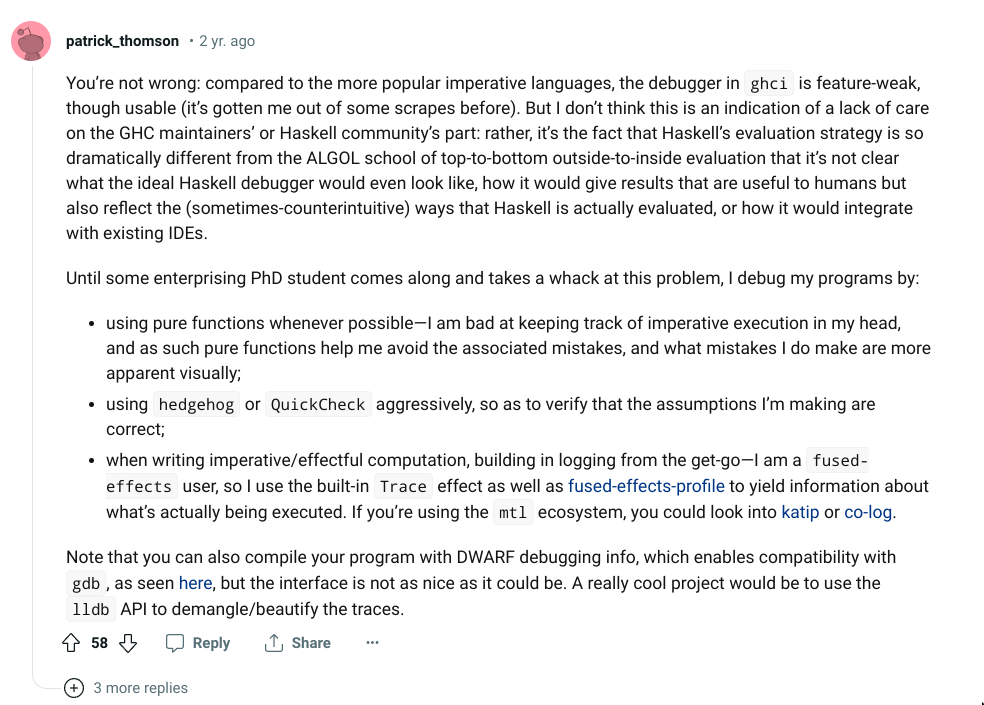
\includegraphics[width=\linewidth]{snapshots/haskell_debugging_is_hard01.png}
\end{frame}

\begin{frame}
	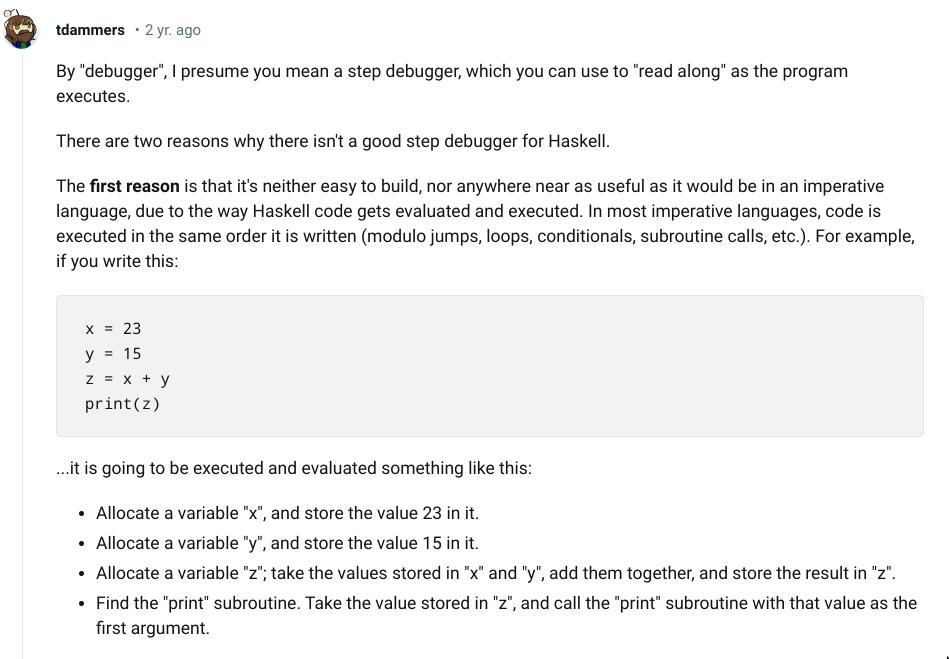
\includegraphics[width=\linewidth]{snapshots/haskell_debugging_is_hard02.png}
\end{frame}

\begin{frame}
	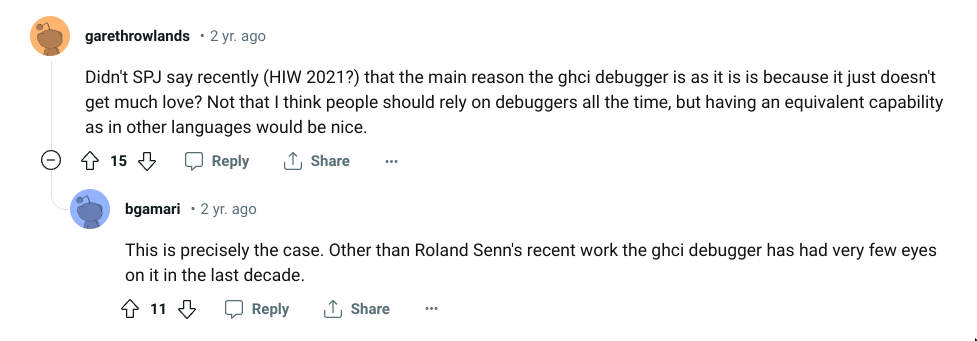
\includegraphics[width=\linewidth]{snapshots/haskell_debugging_is_hard03.png}
\end{frame}

\section{Regular Feautures}
\begin{frame}
\frametitle{Regular Features}
This section we will discuss the regular features of Husky.

\begin{itemize}
	\item functions
	\item methods
	\item values
	\item type definitions
\end{itemize}
\end{frame}

\begin{frame}
\frametitle{Item}
\end{frame}

\begin{frame}
\frametitle{Type Definition}

One can define
\begin{itemize}
	\item regular struct/structure
	\item tuple struct/structure
	\item unit struct/structure
	\item enum/inductive
	\item 
\end{itemize}

Here struct enum are for runtime values, and structure or inductive are for compile time (term level) values. The details are yet to be determined.
\end{frame}

\begin{frame}
\frametitle{Variance}
Basically the same as Rust.

Of course, having variance makes type inference more complicated, but I have the time.
\end{frame}

\begin{frame}
\frametitle{Place and At Type}
Rust introduces the concept of \textcolor{orange}{lifetime}, so does Husky, but Husky also introduces \textcolor{orange}{place}. 

{\color{gray}Afterall, time and space is the same thing according to Einstein.}
\end{frame}

\begin{frame}
\frametitle{Place and At Type}
For linear link list, Husky can do without unsafe, but Rust can't.
\end{frame}

\begin{frame}
\frametitle{Borrow Checking}
In Rust, lifetime is tied to a region, which limits its expressive power. In Husky I've invented a better way of checking, maybe also more efficient, enabling more safe code to pass borrow checking.

{\color{gray}However, I have seen a paper from Germany that looks like doing similar things.}

In Husky, I just collect all lifetime constraints and simply run a `symbolic simulation' to detect lifetime conflicts, with special handles for branches and loops. Unfortunately, they are implemented only in the old C++ codebase, I've not yet got time to do that in the current Rust codebase.
\end{frame}

\begin{frame}
\frametitle{Decorators}
must\_use, no\_discard

\end{frame}

\begin{frame}
\frametitle{Monad through Effect and Unveil}
\end{frame}

\begin{frame}
\frametitle{Incremental Code Analysis}
\end{frame}

\begin{frame}
\frametitle{Regular Features: Incremental Compilation}
\end{frame}

\begin{frame}
\frametitle{Regular Features: Affine Type}
\end{frame}

\begin{frame}
\frametitle{Regular Features: Lifetime and Place}
\end{frame}

\begin{frame}
\frametitle{Regular Features: Generics}
\end{frame}

\begin{frame}
\frametitle{Regular Features: Dependent Types}
\end{frame}

\section{Development Progress}

\begin{frame}
\frametitle{Agility}
\begin{itemize}
	\item What I don't like is, run into stable version and then discover the features don't satisfy the needs.
	\item Agility: keep language unstable, test it for various tasks, and gradually adapt.
	\item 5-10 years from version 0.1, 15-20 years from version 1.0.
	\item Good enough to apply it for AI research within months.
	\item For production, transpile into C or Zig or even high level C++ or Rust.
\end{itemize}
\end{frame}

\begin{frame}
\frametitle{Solo Project}

So far it has been only me.

\begin{itemize}
	\item 
\end{itemize}
\end{frame}

\begin{frame}
\frametitle{Community}

The community should be kept very small for the language development to be agile.
\begin{itemize}
	\item AI researchers.
	\item Game developers.
	\item UI
	\item students
\end{itemize}
\end{frame}
\end{document}